\documentclass{article}

\usepackage{tikz}
\usetikzlibrary{arrows,calc,fit}
\tikzset{box/.style={draw, rectangle, rounded corners, thick, node distance=7em, text width=6em, text centered, minimum height=3.5em}}
\tikzset{container/.style={draw, rectangle, dashed, inner sep=2em}}
\tikzset{line/.style={draw, thick, -latex'}}

\begin{document}

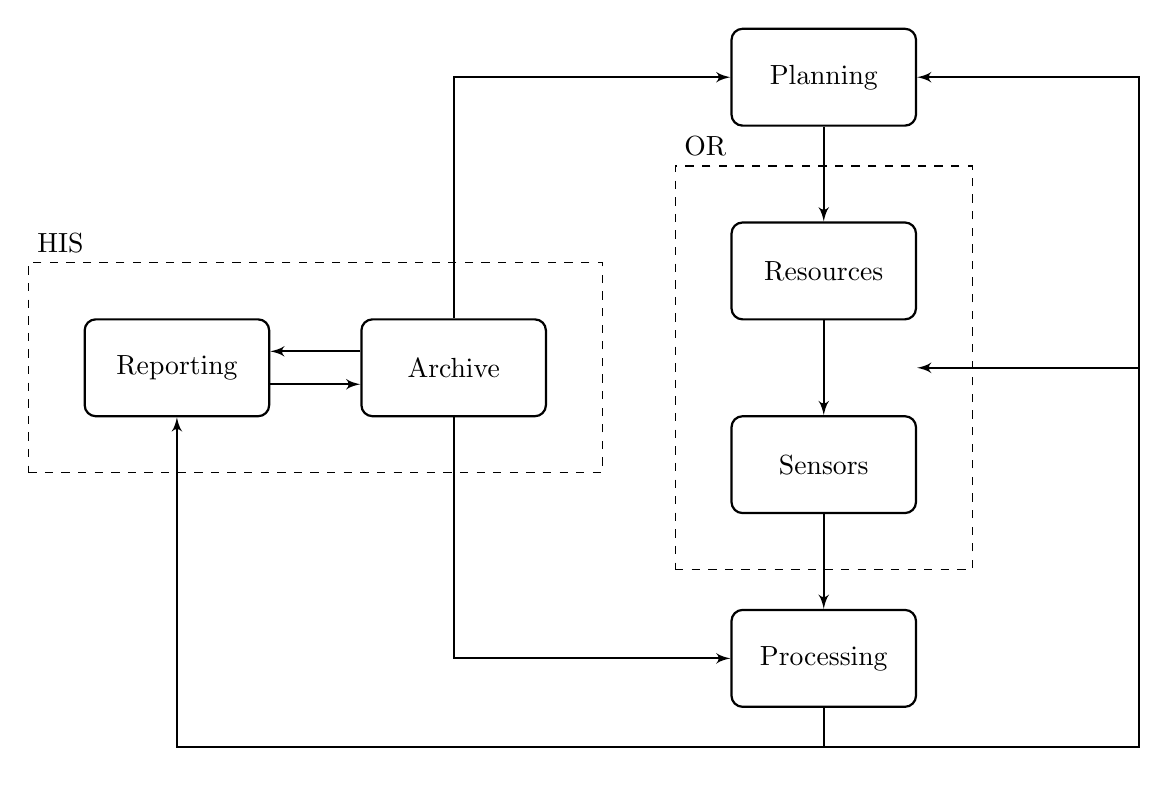
\begin{tikzpicture}[auto]
    \node [box] (planning) {Planning};
    \node [box, below of=planning] (resources) {Resources};
    \node [box, below of=resources] (sensors) {Sensors};
    \node [box, below of=sensors] (processing) {Processing};

    \coordinate (middle) at ($(resources.west)!0.5!(sensors.west)$);
    \node [box, left of=middle, node distance=10em] (archive) {Archive};
    \node [box, left of=archive, node distance=10em] (reporting) {Reporting};

    \node[container, fit=(resources) (sensors)] (or) {};
    \node at (or.north west) [above right,node distance=0 and 0] {OR};

    \node[container, fit=(archive) (reporting)] (his) {};
    \node at (his.north west) [above right,node distance=0 and 0] {HIS};

    \path [line] (planning) -- (resources);
    \path [line] (resources) -- (sensors);
    \path [line] (sensors) -- (processing);

    \path [line] (archive) |- (planning);
    \path [line] (archive) |- (processing);
    \path [line] (processing)--($(processing.south)-(0,0.5)$) -| (reporting);

    \draw [line] ($(processing.south)-(0,0.5)$) -- ++(4,0) node(lowerright){} |- (planning.east);
    \draw [line] (lowerright |- or.east) -- (or.east -| resources.south east);

    \draw[line] (archive.170)--(reporting.10);
    \draw[line] (reporting.350)--(archive.190);
\end{tikzpicture}

\end{document}
